\documentclass[11pt]{article}

% Basic packages
\usepackage[utf8]{inputenc}
\usepackage[T1]{fontenc}
\usepackage{lmodern}
\usepackage{xcolor}
\usepackage{graphicx}
\usepackage{listings}
\usepackage[breakable,skins,theorems]{tcolorbox}
\usepackage{titlesec}
\usepackage{caption}
\usepackage{fancyhdr}  % Add this for footer control
\usepackage{enumitem}  % Add this package for itemize options

% Set page dimensions - custom height of 400mm
\usepackage[paperwidth=210mm,paperheight=370mm,top=1cm,bottom=2cm,left=1cm,right=1cm]{geometry}

% Color definitions
\definecolor{commandcolor}{rgb}{0.8,0.0,0.0}
\definecolor{commentcolor}{rgb}{0.4,0.8,0.4}
\definecolor{sectioncolor}{rgb}{0.0,0.3,0.5}
\definecolor{subsectioncolor}{rgb}{0.0,0.4,0.4}
\definecolor{subsubsectioncolor}{rgb}{0.0,0.5,0.7}
\definecolor{warningcolor}{rgb}{0.9,0.5,0.3}
\definecolor{kalibackground}{rgb}{0.15,0.15,0.15}
\definecolor{kalitext}{rgb}{0.4,0.7,1.0}
\definecolor{codebackground}{rgb}{0.95,0.95,0.95}

% Custom environments
\newenvironment{commandbox}[1][]{
  \begin{tcolorbox}[
      colback=kalibackground,
      colframe=commandcolor,
      fonttitle=\bfseries\color{white},
      title=#1,
      breakable=true
    ]
  }{
  \end{tcolorbox}
}

% Code listing settings
\lstset{
  backgroundcolor=\color{kalibackground},
  basicstyle=\footnotesize\ttfamily\color{warningcolor},
  breaklines=true,
  commentstyle=\color{commentcolor},
  keywordstyle=\color{kalitext},
  stringstyle=\color{kalitext}
}

\lstdefinestyle{bash}{
  morecomment=[l][\color{commentcolor}]{\#}
}

% Section formatting
\titleformat{\section}
{\color{sectioncolor}\normalfont\Large\bfseries}
{\color{sectioncolor}\thesection}{1em}{}

\titleformat{\subsection}
{\color{subsectioncolor}\normalfont\large\bfseries}
{\color{subsectioncolor}\thesubsection}{1em}{}

\titleformat{\subsubsection}
{\color{subsubsectioncolor}\normalfont\normalsize\bfseries}
{\color{subsubsectioncolor}\thesubsubsection}{1em}{}

% Set up fancy headers/footers
\pagestyle{fancy}
\fancyhf{}  % Clear all header/footer fields
\renewcommand{\footrulewidth}{0pt}  % No footer rule
\renewcommand{\headrulewidth}{0pt}  % No header rule

% This pushes the page number to the bottom of the page
\fancyfoot[R]{\vspace*{350mm}Page \thepage}

\begin{document}

\setcounter{section}{3}
\setcounter{page}{13}  % Set the page number appropriately

% Add this to make subsubsection use Roman numerals
\renewcommand{\thesubsubsection}{\thesubsection.\Roman{subsubsection}}

\section{Basic Port Scanning}

\begin{tcolorbox}[colback=codebackground, colframe=warningcolor]
  So far when we scanned ports we've seen only the \textbf{Open}
  state, but here's what Nmap also considers:

  \begin{itemize}[leftmargin=*]
    \item \textbf{Open}: indicates that a service is listening on the
      specified port.
    \item \textbf{Closed}: indicates that no service is listening on
      the specified port, although the port is accessible. By
      \textit{accessible}, we mean that it is reachable and is not
      blocked by a firewall or other security appliances/programs.
    \item \textbf{Filtered}: means that Nmap cannot determine if the
      port is open or closed because the port is not accessible. This
      state is usually due to a firewall preventing Nmap from
      reaching that port. Nmap's packets may be blocked from reaching
      the port; alternatively, the responses are blocked from
      reaching Nmap's host.
    \item \textbf{Unfiltered}: means that Nmap cannot determine if
      the port is open or closed, although the port is accessible.
      This state is encountered when using an ACK scan \texttt{-sA}.
    \item \textbf{Open|Filtered}: This means that Nmap cannot
      determine whether the port is open or filtered.
    \item \textbf{Closed|Filtered}: This means that Nmap cannot
      decide whether a port is closed or filtered.
  \end{itemize}
\end{tcolorbox}
\begin{center}
  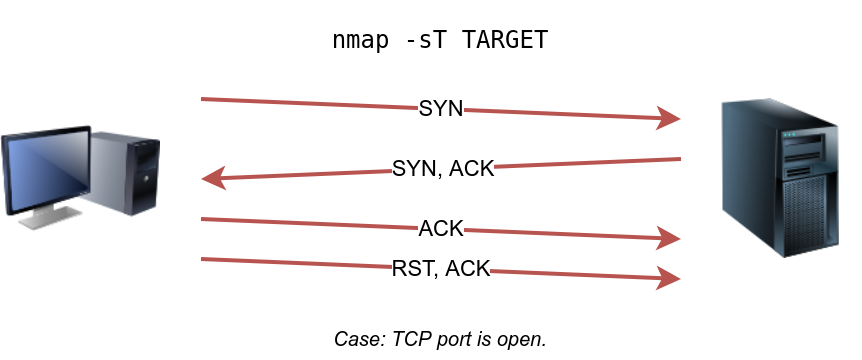
\includegraphics[width=0.7\textwidth]{st-discovery.png}
  \captionof{figure}{A closed TCP port responds to a SYN packet with
  RST/ACK to indicate that it is not open.}
  \label{fig:sT-scan}
\end{center}
\begin{center}
  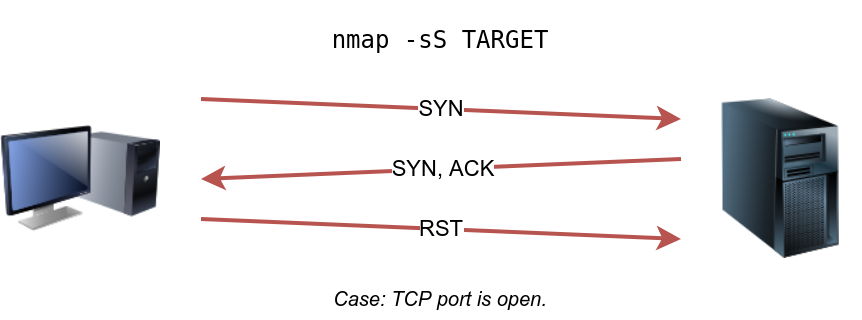
\includegraphics[width=0.7\textwidth]{stealth-scan.png}
  \captionof{figure}{SYN scan does not need to complete the TCP 3-way
    handshake; instead, it tears down the connection once it receives a
  response from the server.}
  \label{fig:sS-scan}
\end{center}

\begin{center}
  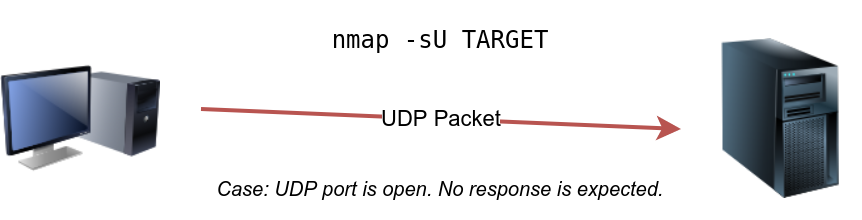
\includegraphics[width=0.7\textwidth]{sU-success.png}
  \captionof{figure}{the UDP ports that don’t generate any response
  are the ones that Nmap will state as open.}
  \label{fig:sU-scan-success}
\end{center}
\begin{center}
  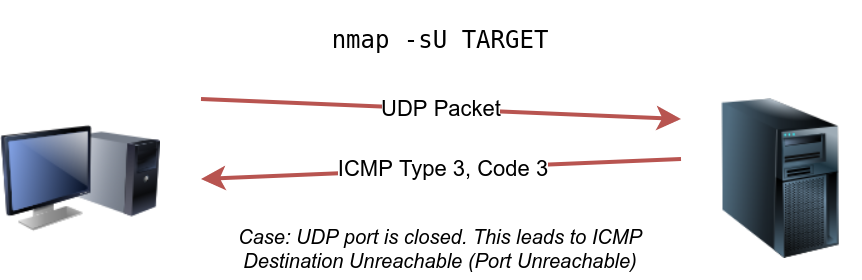
\includegraphics[width=0.7\textwidth]{sU-failed.png}
  \label{fig:sU-scan-failure}
\end{center}
\end{document}
